% Template for Cogsci submission with R Markdown

% Stuff changed from original Markdown PLOS Template
\documentclass[10pt, letterpaper]{article}

\usepackage{cogsci}
\usepackage{pslatex}
\usepackage{float}
\usepackage{caption}

% amsmath package, useful for mathematical formulas
\usepackage{amsmath}

% amssymb package, useful for mathematical symbols
\usepackage{amssymb}

% hyperref package, useful for hyperlinks
\usepackage{hyperref}

% graphicx package, useful for including eps and pdf graphics
% include graphics with the command \includegraphics
\usepackage{graphicx}

% Sweave(-like)
\usepackage{fancyvrb}
\DefineVerbatimEnvironment{Sinput}{Verbatim}{fontshape=sl}
\DefineVerbatimEnvironment{Soutput}{Verbatim}{}
\DefineVerbatimEnvironment{Scode}{Verbatim}{fontshape=sl}
\newenvironment{Schunk}{}{}
\DefineVerbatimEnvironment{Code}{Verbatim}{}
\DefineVerbatimEnvironment{CodeInput}{Verbatim}{fontshape=sl}
\DefineVerbatimEnvironment{CodeOutput}{Verbatim}{}
\newenvironment{CodeChunk}{}{}

% cite package, to clean up citations in the main text. Do not remove.
\usepackage{apacite}

% KM added 1/4/18 to allow control of blind submission


\usepackage{color}

% Use doublespacing - comment out for single spacing
%\usepackage{setspace}
%\doublespacing


% % Text layout
% \topmargin 0.0cm
% \oddsidemargin 0.5cm
% \evensidemargin 0.5cm
% \textwidth 16cm
% \textheight 21cm

\title{A Language's Unigram Entropy Distribution Predicts Self-Paced Reading
Times}


\author{{\large \bf Josef Klafka} \\ \texttt{jklafka@uchicago.edu} \\ Department of Psychology \\ University of Chicago \And {\large \bf Daniel Yurovsky} \\ \texttt{yurovsky@uchicago.edu} \\ Department of Psychology \\ University of Chicago}

\begin{document}

\maketitle

\begin{abstract}
We provide evidence against the Uniform Information Density (Jaeger,
2010) and wrap-up effect hypotheses.

\textbf{Keywords:}
Entropy; self-paced reading; information theory; language processing
\end{abstract}

\section{Uniform Information Density}\label{uniform-information-density}

How do people convey information in speech and text? Is there a regular
distribution to how information is conveyed across speech and text? Does
speech, with its phonological properties, different from writing, with
its semiotic properties, in how information is conveyed?

A major line of research in the current century has asked how speakers
and writers distribute information in the linguistic material they
produce. This begins with Claude Shannon in the years after World War
II. Shannon (1948) defined ``information'' as a ``reduction in
uncertainty''. Shannon followed by quantifying uncertainty in his
measure of \emph{entropy}: the amount of uncertainty on the outcome of a
random variable. Shannon proposed that the most efficient method of
sending information through a noisy channel is at a constant rate.
Genzel \& Charniak (2002) apply this principle to human communication:
if people communicate information through speech and text optimally,
then we should transmit information to one another at a constant rate.
Genzel \& Charniak created a distribution of estimates for
sentence-level entropy, each sentence taken without context, for
newspaper articles from the Penn Treebank corpus. Obtaining a roughly
monotonically increasing linear distribution, Genzel \& Charniak
proposed the \emph{Constant Entropy Rate} (CER) principle: the entropy
rate in speech and text with context should be constant as sentence
number increases. Aylett \& Turk (2004) proposed a similar principle for
the phonological level.

Jaeger (2010) extends the CER principle to all levels of human
communication: the \emph{Uniform Information Density} (UID) hypothesis.
Jaeger argues that speakers will try to distribute information more
evenly over the course of an utterance, to be as close to channel
capacity (in a Shannon sense) as possible. In particular, Jaeger singles
out the production of ``that'' at the beginning of relative clauses in
English and the use of contractions such as ``he's'' and ``you're''
versus ``he is'' and ``you are'' as instances where higher information
density in the clause elicits the production of more material by
speakers.

The UID hypothesis

\subsection{UID challenges}\label{uid-challenges}

More recent work has stood out in contrast to the traditional UID
perspective. Zhan and Levy (2018) study Mandarin Chinese classifier use,
and find that the use of specific classifier, versus general
classifiers, appears more often in cases where the production of the
corresponding noun is more difficult than when the production is easier,
as would be predicted by UID. The UID perspective is challenged in Yu et
al. (2016), by performing an analysis of entropy by position in the text
portion of the British National Corpus. They use the following formula
for each word position X of sentences of fixed length k from the corpus,
where each i is a word occurring in position X and pi is the number of
times word i occurs in position X divided by the number of total words
that occur in position X i.e.~the number of sentences of length k.

\[H(X) = \sum\limits_w p(w)\log\big(p(w)\big)\] Yu et al. (2016) refer
to their distribution for English as a `three-step distribution':
relatively low entropy at the beginning of a sentence, then a jump, then
flat entropy in the middle, a dip before the final position and a jump
with the final word. View the figure below for a visual demonstration.

\section{Methods}\label{methods}

We used the CHILDES TalkBank (Brown 1973; MacWhinney 2000) corpora
database of spoken adult-child conversations. We first used the Brown
and Providence English corpora from CHILDES. The Brown corpus contains
conversations between three young children (over 1.5 years old and under
6 years old) and their families in the home. The Providence corpus
contains transcriptions of audio/video files which recorded interactions
between children between 1 and 3 years old and their parents in the
home. We divided each corpus by speaker into child and non-child
categories. We further divided the corpora by utterance length, so that
all sentences of length \(k\) (e.g. \(6\)) were grouped together.
Finally, within each utterance length, we computed the unigram entropy
measure for each position.

The unigram entropy measure works as

Figure for the method?

Plots for the entropy distributions are below. The adult and child
unigram entropy distributions track one another extremely well, with the
child distribution for each sentence length having relatively lower
entropy.

\begin{CodeChunk}
\begin{figure*}[h]

{\centering 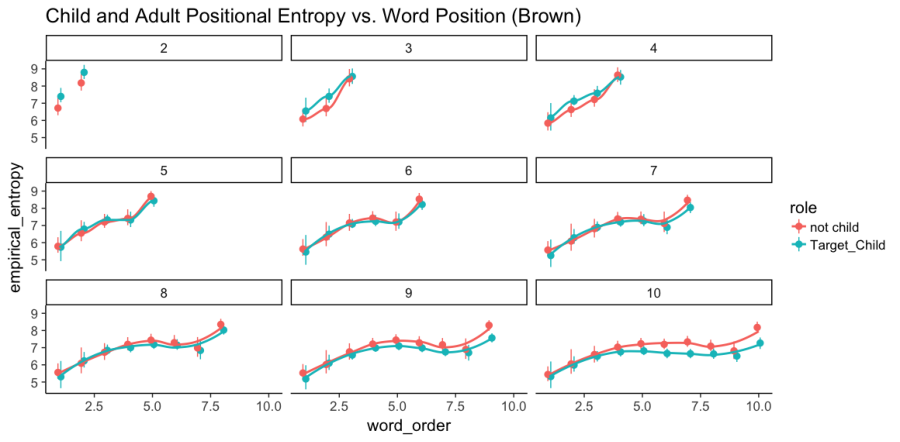
\includegraphics{figs/brown_PE-1} 

}

\caption[Brown corpus entropy]{Brown corpus entropy}\label{fig:brown_PE}
\end{figure*}
\end{CodeChunk}

\begin{CodeChunk}
\begin{figure*}[h]

{\centering 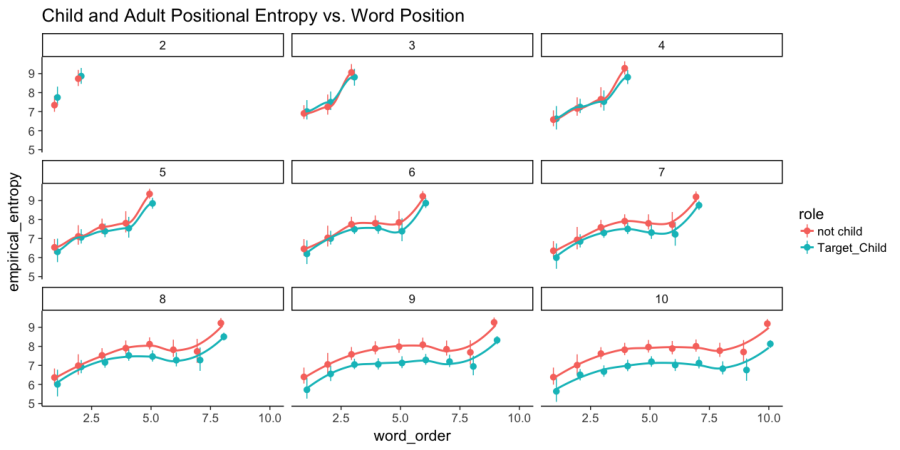
\includegraphics{figs/providence_PE-1} 

}

\caption[Providence corpus unigram entropy]{Providence corpus unigram entropy}\label{fig:providence_PE}
\end{figure*}
\end{CodeChunk}

We also ran this analysis on Spanish, German, Mandarin and Japanese
corpora from CHILDES. The Spanish corpus we used was the XXX and the
German corpus we used was the XXX. The Mandarin corpus we used was the
XXX and the Japanese corpus we used was the XXX. For Mandarin, we used
pinyin transliterations of the utterances in the corpus with demarcated
word boundaries, and for Japanese we used romanji transliterations of
words in the corpus. Japanese Hiragana, Katakana and Kanji writing
systems, and the Chinese characters used for writing Mandarin do not
normally demarcate word boundaries by spacing words apart, and for
normal Japanese and Chinese writing including spaces between word
boundaries can have a negative effect on reading times (Sainio et al,
2007; Bai et al, 2008).

\section{Results}\label{results}

We found a distinct three-step distribution for English, Spanish and
German CHILDES corpora, with a slight dip in the penultimate position of
each sentence. The Mandarin and Japanese data, by comparison,

\section{Analysis}\label{analysis}

\section{Wikipedia Data}\label{wikipedia-data}

We also wanted to apply this analysis to large-scale text data, to
compare with the parent-child speech data results from using CHILDES.
Using Giuseppe Attardi's Wikiextractor tool
\footnote{https://github.com/attardi/wikiextractor}, we extracted the
text corpora for \(165\) languages from Wikipedia by downloading the
data dump of Wikipedia. Each language corpus was cleaned and limited to
sentences between \(6\) and \(50\) words. Similar to the data from
CHILDES, we divided each corpus by sentence length, and then computed
the unigram entropy measure on each word position within each sentence
length. HOW DID WE JOIN TOGETHER SENTENCE LENGTHS

\subsection{Clustering}\label{clustering}

\section{Conclustions and future
research}\label{conclustions-and-future-research}

The \emph{wrap-up effect} is a popular hypothesis within the
eye-tracking community. The hypothesis states that, in written text,
sentence-final words are processed more slowly on average then
sentence-medial or sentence-initial words, due to readers integrating
information from the entire sentence in order to form a final, coherent
thought expressed by the sentence, among other reasons. With these two
ideas, information production distribution in spoken and written
communication, and information integration in reading written texts, we
move on to discuss cross-linguistic differences in the distribution of
information across sentences.

\section{Acknowledgements}\label{acknowledgements}

Place acknowledgments (including funding information) in a section at
the end of the paper.

\section{References}\label{references}

\setlength{\parindent}{-0.1in} \setlength{\leftskip}{0.125in} \noindent

\bibliographystyle{apacite}


\end{document}
